\chapter{nRF24L01p}
\noindent

\section{Introdução ao nRF24L01+}
\paragraph{} O nRF24L01+ é um transceptor de chip único que opera na faixa ISM de 2.4 GHz com o protocolo Enhanced ShockBurst\textsuperscript{TM} incorporado. O chip é produzido pela Nordic Semiconductor, localizada na Noruega, que é especializada em sistemas sem fio de baixo consumo de energia em um chip (SoC) \citep{Nordic2008}.

\paragraph{} Seu funcionamento depende de um microcontrolador, e a sua configuração é feita através de uma interface serial periférica (SPI).


\paragraph{} O módulo usado no projeto é o E01-ML01DP5 da EBYTE. Esse módulo contém o chip nRF24L01+ da Nordic e um amplificador de potência de 20 dBm e um \textit{Low Noise Amplifier}. O módulo apresenta largura de 18 mm e comprimento de 43 mm (conforme a figura \ref{fig:figura52}. A Chengdu Ebyte Eletronic Technology foi criada na China e é uma empresa de alta tecnologia especializada em comunicações da Internet das Coisas (IoT)\citep{EBYTE}.

\paragraph{} O nRF24L01+ tem diversas aplicações como mouse, teclados, controles remotos, sensores e automação domiciliar.

\begin{figure}[!ht]
	\centering
	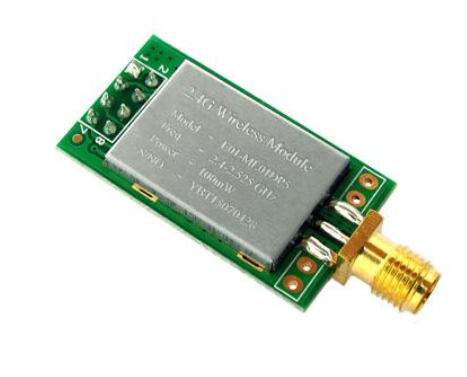
\includegraphics[width=0.4\textwidth]{Figuras/nrf24.PNG}   
	\caption{Módulo E01-ML01DP5 da EBYTE. \citep{EBYTE}}
	\label{fig:figura52}
\end{figure}


\section{Parâmetros}
\paragraph{} Para a realização da transmissão e recepção no projeto, foram usados os seguintes parâmetros do módulo E01-ML01DP5:

\begin{table}[ht]
\centering
\caption{Parâmetros do E01-ML01DP5 para o projeto.}
\vspace{0.5cm}
\begin{tabular}{r|lr}

Banda de operação & 2.400 GHz a 2.525 GHz \\
\hline
Modulação & GFSK \\
Taxa de bits & 250 \\
Potência de transmissão máxima & 20 dBm \\
Sensibilidade do receptor & -106 dBm \\
Número de canais & 126 \\
Largura de banda & 700 KHz \\
Desvio de frequência & 160 kHz \\
Alcance máximo & 2100 m
 
\end{tabular}
\label{tab:tabela2}
\end{table}

\section{\textit{MultiCeiver}}
\paragraph{} \textit{MultCeiver} é um recurso do nRF24L01+ que permite que  o receptor possa receber pacotes de até 6 endereços diferentes em paralelo, enquanto um transmissor poderá enviar apenas para 1 endereço (conforme a figura \ref{fig:figura50}). 

\begin{figure}[!ht]
	\centering
	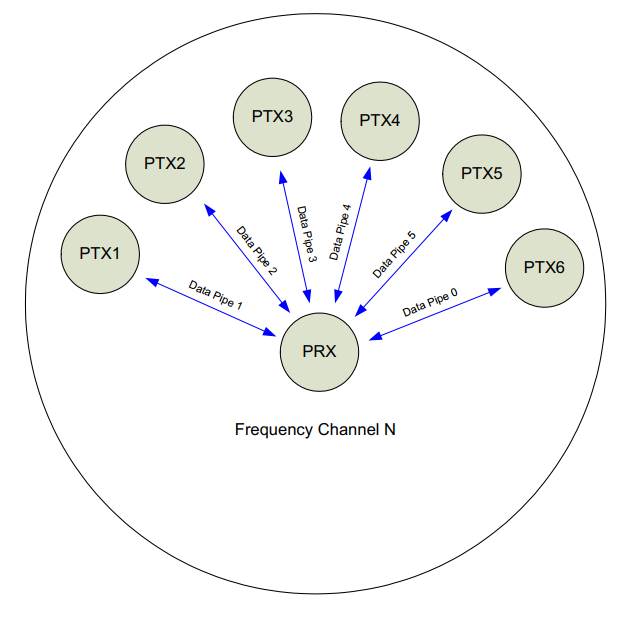
\includegraphics[width=0.4\textwidth]{Figuras/multiceiver.PNG}  
	\caption{\textit{MultiCeiver} do nRF24L01+ \citep{Nordic2008}.}
	\label{fig:figura50}
\end{figure}

\paragraph{} Como apenas um canal de dados pode receber um pacote de cada vez, a partir do momento em que um desses canais receber um pacote completo, os outros canais poderão passar a receber dados. 

\section{Estrutura dos Pacotes (Enhanced ShockBurst\textsuperscript{TM})}
\paragraph{} O pacote do nRF24L01+ segue o formato do protocolo Enhanced ShockBurst\textsuperscript{TM} que divide o pacote em preâmbulo, endereço, \textit{Packet Control}, \textit{payload} e CRC, conforme na figura \ref{fig:figura51}: 

\begin{figure}[!ht]
	\centering
	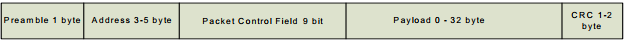
\includegraphics[width=0.7\textwidth]{Figuras/pacote_nrf24.PNG}   
	\caption{Modelo de pacote Enhanced ShockBurst\textsuperscript{TM}.\citep{Nordic2008}}
	\label{fig:figura51}
\end{figure}

\paragraph{} O preâmbulo, que serve para treinar o equalizador, apresenta um número suficiente de transições para estabilizar o receptor. Nesse formato de pacote, o preâmbulo tem apenas 1 byte contendo "10101010" se o primeiro bit do endereço for 1, ou 1 byte contendo "01010101" se o primeiro bit do endereço for 0.

\paragraph{} O segundo campo é o de endereço do receptor, ele pode ser configurado para ter de 3 a 5 bytes de tamanho. 

\paragraph{} O campo do \textit{Packet Control} apresenta 9 bits, sendo que os 6 primeiros são para definição do tamanho do payload (de "000000" a "100000"), os outros 2 bits são de \textit{Packet identification} (PID), e o último bit é para o \textit{No Acknowledgment flag} (NO\_ACK). O PID é um detector de pacote repetido, se o PID e o CRC do pacote forem iguais aos do anterior, esse pacote é considerado uma cópia e, portanto, é descartado. O nono bit do \textit{Packet Control} define se o transmissor receberá, ou não, um pacote de confirmação de recebimento.

\paragraph{} O \textit{Payload} tem tamanho dinâmico de acordo com o definido no \textit{Packet Control} e varia de 0 a 32 bytes.

\paragraph{} Por fim, o pacote disponibiliza um código CRC de 8 ou 16 bits no formato ITU-T, como citado anteriormente no capítulo 3.3.2.3 o polinômio gerador utilizado será o de 16 bits. Esse campo será preenchido com o resto da divisão da sequência de bits \textit{Packet Control} + \textit{Payload} pelo polinômio gerador.